\subsection{虚拟文件系统}
Linux虚拟文件系统隐藏底层物理文件系统的实现,
把支持的所有文件系统通过一个通用文件模型({\em common file model})
严格地按传统{\sc Unix}方式呈现给应用层。
其实现的最主要思想是将文件系统的各个部分封装为对象,
对文件系统各部分的操作则通过函数指针的方式声明为该对象的抽象方法,
方法的具体实现由物理文件系统完成。
通用文件系统模型主要的对象有:

\begin{itemize}
\item[{\em super block}]:这类对象用于描述已挂载的文件系统,
  如果是磁盘文件系统,
  一般对应于存储在磁盘某个固定位置的用于描述整个文件系统的控制块
  ({\em filesystem control block})
\item[{\em inode}]:一个inode类型对象描述唯一的一个文件,
  如果是磁盘文件系统,
  它对应存储在磁盘上的文件的元数据,
  即文件控制块({\em file control block}),
  每一个inode有一个唯一的标识号
\item[{\em dentry}]:这类对象在一条目录项(文件名)和一个文件之间建立关联,
  这种关联在磁盘文件系统中持久存储在磁盘中,
\item[{\em file}]:这类对象描述某个进程打开的文件,
  用于完成进程和打开文件之间的交互,
  只存在于内核内存中。
  每一个打开的文件都有一个进程内唯一号,
  称为文件描述子({\em file descriptor, fd}),
  这个唯一号用于索引文件对象数组。
\end{itemize}

这些对象的联接关系图\,\ref{fig:vfs_obj}:
\begin{figure}[!ht]
  \centering
  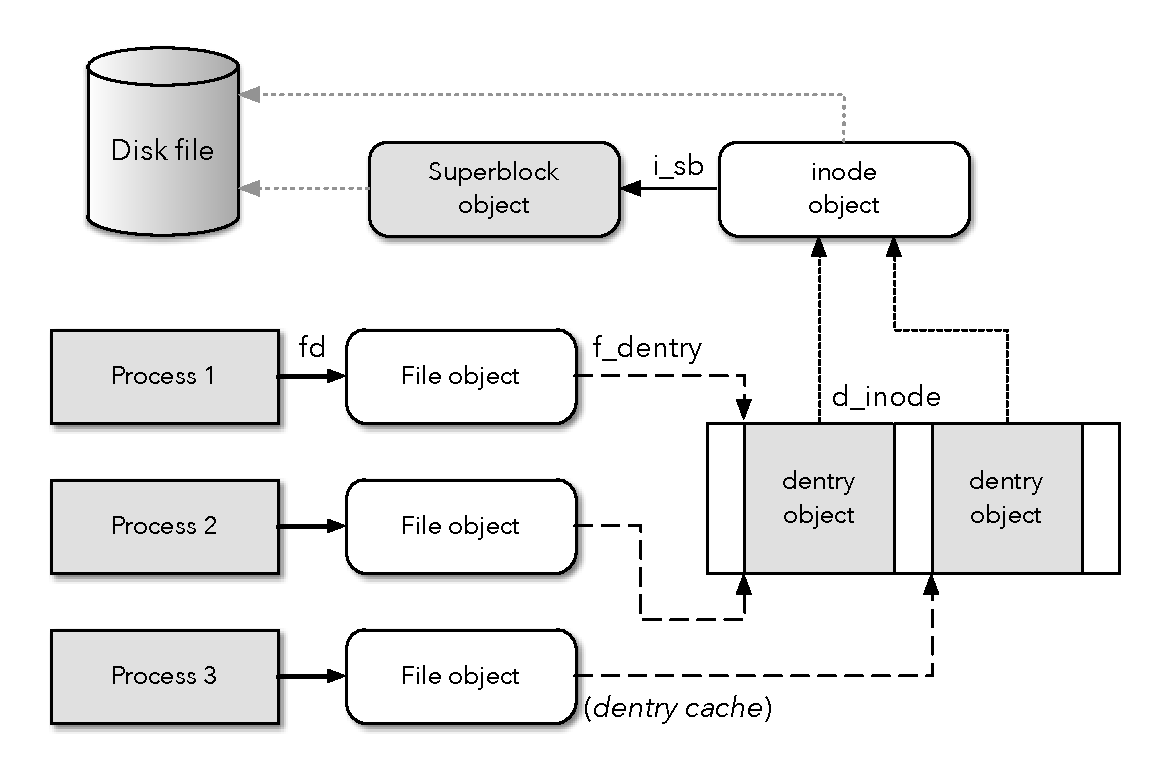
\includegraphics[width=\textwidth]{fig/vfs_objects.pdf}
  \caption{虚拟文件系统各对象关系}
  \label{fig:vfs_obj}
\end{figure}

\subsubsection{Superblock}
Superblock是整个文件系统的控制数据结构,
内存中结构的某些域在磁盘上有永久存储的映像。
Linux超级块由\struct{super\_block}表示,
其中几个重要的域包括
\struct{s\_blocksize}(文件系统块大小)、
\struct{s\_type}(文件系统类型描述子)、
\struct{s\_maxbytes}(最大文件尺寸)、
\struct{s\_dirty}(改动过的inode链表)、
\struct{s\_op}(超级块方法)、
\struct{s\_fs\_info}(对应物理文件系统超级块信息)等等。
出于效率考虑,
物理文件系统超级块\struct{s\_fs\_info}通常会在内存中缓存,
一旦出现对超级块的改动,
域\struct{s\_dirt}被置,
超级块在未来某个时候会被更新到磁盘上。

超级块的方法除了对超级块本身的操作
(\func{put\_super}、\func{write\_super})之外,
最重要的就是对inode的分配、释放、和修改
(\func{alloc\_inode}、\func{destroy\_inode}、
  \func{dirty\_inode}、\func{write\_inode})等等。
有趣的是超级块方法中没有从磁盘读入超级块的\func{get\_sb},
这其实是合逻辑的,
因为超级块的读入显然要先于超级块对象存在,
即需要一层逻辑处于超级块之外的软件完成将超级块从磁盘读入,
这一功能由\struct{filesystem}类型的\func{get\_sb}方法完成。

\subsubsection{inode}
inode对象是文件的控制块,
和文件一一对应,
磁盘文件系统的inode显然需要永久存储映像。
重要的域如下表所示:

\begin{table}[ht]
  \centering
  \begin{tabular*}{0.755\textwidth}{lll}
    \hline
    类型 & 域 & 描述\\  
    \hline
    \struct{unsigned long} & \struct{i\_ino} & inode number\\
    \struct{struct timespec} & \struct{i\_atime} & 最后访问时间\\
    \struct{struct timespec} & \struct{i\_mtime} & 最后写入时间\\
    \struct{struct timespec} & \struct{i\_ctime} & 最后修改时间\\
    \struct{unsigned long} & \struct{i\_blksize} & 文件块尺寸\\
    \struct{unsigned long} & \struct{i\_blocks} & 文件块数\\
    \struct{unsigned long} & \struct{i\_bytes} & 最后一个块的文件有效字节数\\
    \hline
  \end{tabular*}
\end{table}

\subsection{ext2/3}

\subsection{ZFS 特点}
\subsubsection{Unified Storage}
从IT管理角度,
ZFS 重大特色在于其提供统一的存储系统,
既提供文件系统服务,也提供块设备接口,
即兼具了NAS和SAN的功能,
统一存储系统使得部署和管理存储系统得到简化。

\subsubsection{Data Integrity}
ZFS 的设计最重要关注点是保护数据的完整性,
为实现这个目标,
ZFS 对所有的数据块都计算较验和,
并把较验和存储于用于寻址该数据快的快指针内,
即每个子节点的较验和存于其父节点处。

\subsubsection{Copy-On-Write}
ZFS 的另一大特色在于其数据写入方式。
和常见文件系统采用的块内直接修改不同,
ZFS 采用 COW({\em Copy-On-Write})%
\footnote{不做块内修改的思路来自{Log Structured Filesystem}}
机制写入永久存储介质。
COW 的效果就是直至修改文件系统组织树的根(即,Uberblock)之前,
所做的改动不可见并且源树不会遭到任何修改,
这期间掉电或崩溃不影响源树。
图\,\ref{fig:cow}\,展示了写入某些块的COW过程。

\begin{figure}[!ht]
  \centering
  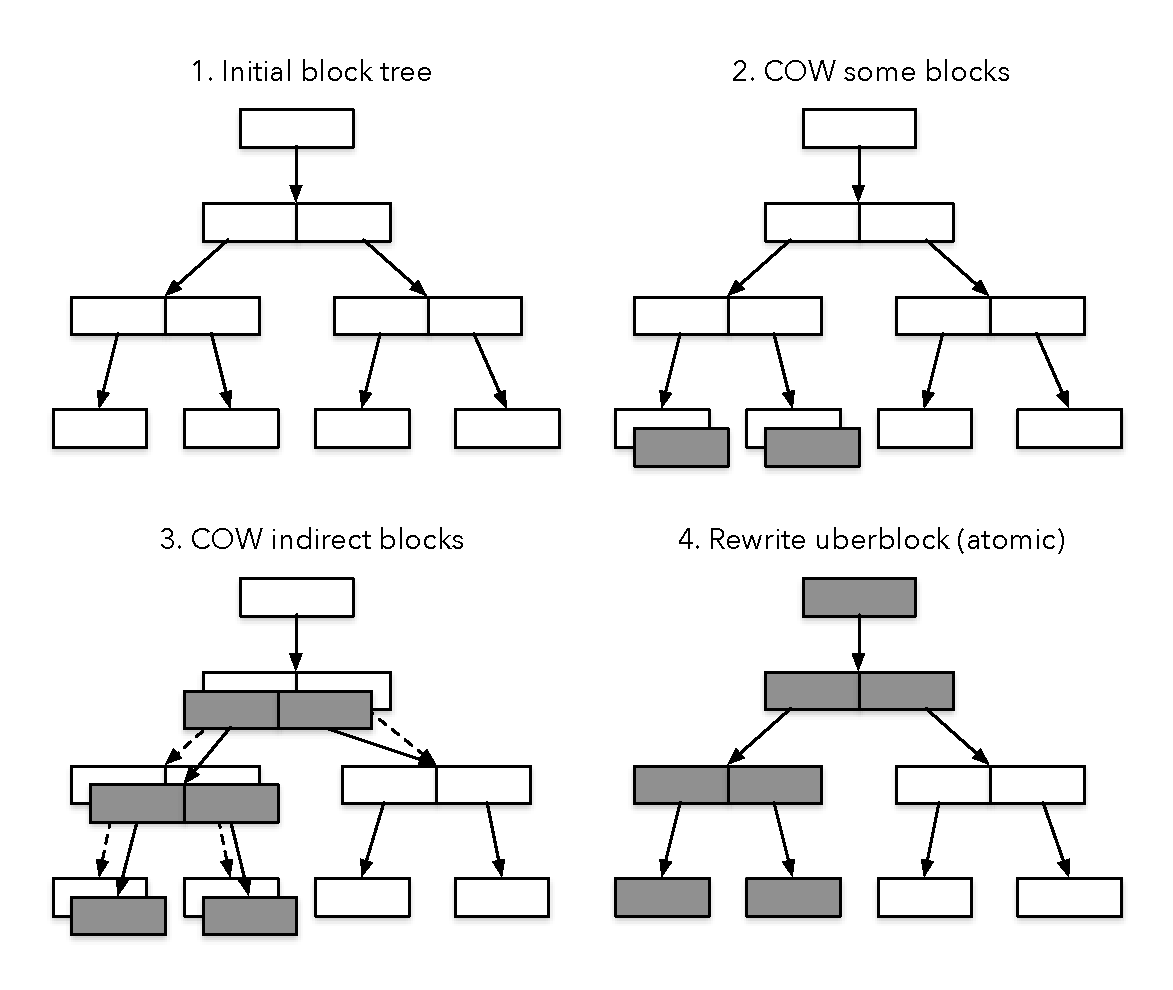
\includegraphics[width=\textwidth]{fig/zfs_cow.pdf}
  \caption{COW}\label{fig:cow}
\end{figure}

传统文件系统当掉电或系统崩溃后极容易出现\emph{文件系统}不一致。
导致不一致问题的本质原因是文件系统的数据更新涉及一系列文件系统内部结构的改动。
譬如对某个文件尾部追加一个数据块,
至少以下的几个步骤要完成:
\begin{enumerate*}[label=\itshape\alph*\upshape)]
  \item 分配一个数据块并写入该数据块;
  \item 修改维护块分配状况的数据结构,位图或B-树等;
  \item 文件的{\em inode}也需要更新,文件长度、修改时间等属性,数据块寻址数据结构。
\end{enumerate*}
这一系列改动可能部分成功部分失败,
并且不保证各部分更新的顺序。
可能有以下几种情况:
\begin{itemize}
  \item 只有数据块分配和写入成功,
    这不是问题,仅仅是刚写入的数据丢失,
    文件系统压根就不知道有这么个数据块存在过;
  \item 只有对inode的更新成功,
    这个后果就严重了,
    \begin{enumerate*}[label=\itshape\alph*\upshape)]
      \item 数据块的指针已写入,而数据未完成,于是从该指针处读出的是垃圾数据
      \item 文件系统的块管理部分未更新,而inode指出某个地址上的块有数据,
        出现文件系统不一致问题;
    \end{enumerate*}
  \item 只有块管理部分得到更新,块管理声明某个块已分配,不能挪作它用,
    但文件系统其它部分又没有使用到它,这称为空间泄漏;
  \item 块管理和inode成功更新而数据未写入,文件系统一致,但用户将得到垃圾数据;
  \item inode和数据写入而块管理未更新,文件系统不一致;
  \item 块管理和数据写入而inode未更新,空间泄漏。
\end{itemize}

传统文件系统通过{\em fsck}工具来解决不一致问题。
\begin{itemize}
  \item fsck从超级块开始,
    检查其正确性,
    如果需要从已知健全的备份超级块恢复;
  \item 而后fsck扫描所有的inode,
    数据块指针,间接快指针,根据它们判断那些块已分配,
    如果和块管理不一致,以inode为准修改块管理数据结构;
  \item fsck试图修正inode的状态,譬如文件类型等属性,
    如果发现inode无法被修正,该inode被丢弃,
    并相应修改块管理数据结构与之匹配;
  \item 修复inode和目录之间链接,
    这通过从根目录开始扫描所有的目录,计算哪些目录项链接到某个inode,
    如果数目不一致,通常修正inode中的链接数;
  \item 一旦发现有多个块指针指向同一块地址,
    如果其中有明显错误,fsck丢弃该块指针,
    否则fsck创建数据块的拷贝,使每个块指针指向自己独享的块;
  \item fsck检查块指针是否合法,譬如其是否指向硬盘分区之外的地址,
    如果块指针被发现不合法,
    fsck能做的最好处理就是从inode或间接指针中删除它;
  \item fsck也修正目录的内容,
    譬如目录``.''和``..''必须是一个目录的头两个目录项
\end{itemize}
可想而知,
fsck的全文件系统扫描机制非常低效。
现代的文件系统引入日志 ({\em journal}) 的概念,
即对文件系统改动之前,
将对更新全过程精确描述先写入存储介质,
当更新过程被意外中断重启系统或重新挂载文件系统时,
可以通过该日志知晓出了什么问题以及如何修复。
一个立刻浮现的问题是,
日志的内容可能很大,
如何保证日志本身的完整性?
答案是只能靠硬件保证。
\footnote{
  题外话,
  现代硬盘不保证多个写入请求按收到的顺序完成,
  即便使用写屏障({\em Write Barrier}) 也有可能被硬件忽略。
}
现代硬盘通常保证一次512字节写入的原子性,
于是日志写入分为两阶段,
\begin{enumerate}
  \item 日志写入,
    即先将日志开始标志和日志内容先写入,这一阶段的原子性无法保证,
    内容写入成功之后,文件系统:
  \item 将日志结束标志原子地写入磁盘
\end{enumerate}
这样一来,日志的完整与否可以由日志结束标志判定。
Linux的Ext4文件系统通过使用较验和实现对日志的一次性写入而不失完整性,
提高了日志写入的效率。
日志文件系统的缺点是任何数据写都要对磁盘操作两次。

回到ZFS,
正因为数据的COW语义,
没有就地修改的数据块,
意外断电或系统崩溃的恶果仅仅是丢失部分未写入数据,
文件系统的一致性得到保障而无需做fsck或日志回放。

\subsubsection{Snapshot \& Clone}
得益于Copy-On-Write机制,
ZFS提供高效的快照({\em Snapshot})和克隆({\em Clone})功能。
对文件系统创建快照之后,
当写入原始文件系统发生COW,
旧数据不会被回收使用,
旧的数据块树将一直存在,
部分新数据和旧数据组成一棵新树,
呈现一个新文件系统。
克隆即可写快照,
所有内容没有被修改过的数据块被共享,
写入克隆文件系统只是导致树产生分杈而不是全部复制。

ZFS文件系统可以被移入另外一个存储池中,
更进一步,
可以被发送到远程。
send命令创建一个流呈现文件系统的状态,
这个流可以呈现某个快照的所有内容,
也可以是两个快照之间的增量,
这提供了一个高效的策略,
用于譬如在HA中同步存储池或者将存储备份至其它主机。

\subsubsection{Transactional Model}
写入请求被归入某个终将写入存储池的事务组中,
事务的含义就是写入以组为原子单位,
ZFS的DMU层不允许部分成功部分失败的情形。
每一个事务组对应文件系统一个一致的状态({\em checkpoint}),
事务组完全写入磁盘后,
即一个checkpoint产生之后,
对uberblock进行一次原子写,
更新事务组号,
于是文件系统跃迁至一个新的、一致的状态上。

\subsubsection{其它}
ZFS还提供数据压缩,加密等用户需要的功能。

ZFS 另外有几个先进的实现,
\begin{description}
  \item[ARC, {\em Adaptive Replacement Cache}]\hfill\\
    ARC 是一个物理页管理算法,效率高于传统的 LRU。
    本质上说 ARC 除了考虑页的使用时间点之外还考虑页的使用频率,
    当需要回收页时,
    ARC算法有效决定从LRU还是LFU链表中选取,
    并动态、自适应地决定两条链的长度。
    除了位于内存中的缓存,
    ZFS引入了二级缓存 ({\em L2ARC}) 的概念,
    将一大部分页缓存放在SSD上免去某些页被换出后需要再次读取而操作磁盘;
  \item[ZIO pipeline]\hfill\\
    将I/O分为20道工序,
    按流水线方式处理,
    使得I/O不同阶段的工序可以在不同的CPU核上完成,
    充分利用多核CPU并行运算能力从而提高吞吐量;
  \item[Space Map]\hfill\\
    实现高效分配、释放存储设备上的块。
\end{description}

\subsubsection{缺点}
COW 的优点是集中了分散的写,
如写不同文件的数据,
又如文件的数据写伴随metadata的写\footnote{数据和元数据往往距离较远},
使它们成为线性写,
大大提高写效率。
但是这产生一个副作用,
文件相邻的块物理上可能非常分散,
造成读效率较低,
这个只能通过大内存做cache和好的缓存算法来适当抵消。

COW 另外一个缺点是会导致碎片,
在磁盘使用率超过70\%,
所有的metaslab都已创建,
其中都或多或少被填充,
文件写入将出现性能瓶颈,
IOPS下降较严重。

\subsection{ZFS组织结构}
一个存储池{\em zpool}是由虚拟设备{\em vdev}节点构成的一棵树。
位于叶端的是负责实际数据存取的物理介质,
故称为{\em phsical vdev};
其余的节点统称为{\em logical vdev},
用于表示 ZFS 的逻辑。
ZFS 藉由抽象的虚拟设备树即可实现不同的Raid级别。

\begin{figure}[ht]
  \centering
  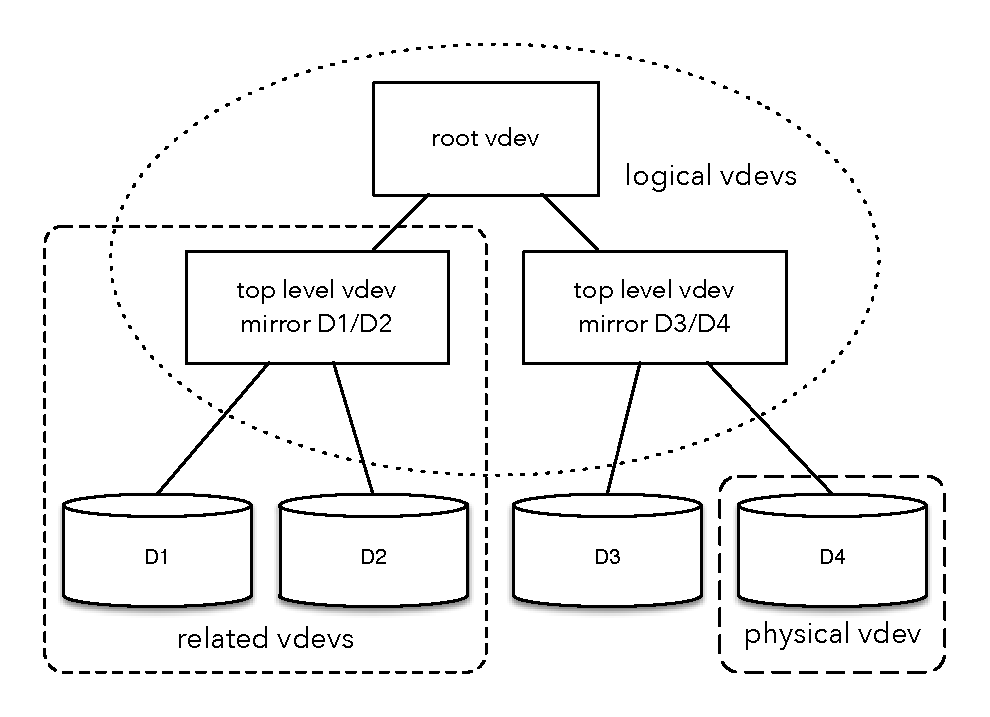
\includegraphics[width=\textwidth]{fig/zfs_architecture.pdf}
  \caption{ZFS架构}\label{fig:arch}
\end{figure}

图\,\ref{fig:arch}\,所表示的存储池结构由如下命令创建,
第二个 mirror 关键字表示将指定新的顶层虚拟设备。
数据通过这两个镜像以动态方式进行条带化,
并会相应地在每个磁盘之间创建冗余数据。
\begin{lstlisting}{lanuage=Bash}
# zpool create tank mirror D1 D2 mirror D3 D4
\end{lstlisting}

\subsection{ZFS代码模块}
从设计实现的角度看,
ZFS 分为 7 个相对独立模块,
模块的简称贯穿整个ZFS文件系统的代码及文档之中。

\begin{description}
  \item[SPL, {\em Storage Pool Allocator}\,:]
    负责存储池一级的操作,如创建,销毁,修改属性等;
  \item[DMU, {\em Data Management Layer}\,:]
    完成将数据块组织为对象,如文件、目录等,
    并且将对象组织为对象集,如文件系统、文件系统快照等;
  \item[DSL, {\em Dataset and Snapshot Layer}:]
    管理对象集属性以及各对象集之间逻辑关系
  \item[ZAP, {\em ZFS Attribute Processor}\,:]
    位于 DMU 层之上,
    操作称为 ZAP 的对象,
    ZAP 对象用于描述如文件系统、存储池等对象集的属性;
  \item[ZPL, {\em ZFS Posix Layer}\,:]
    将 ZFS 的对象、对象集以 Posix 标准的方式呈现,
    提供 POSIX 标准方式的文件操作,如 open、read、write;
  \item[ZIL, {\em ZFS Intent Log}\,:]
    ZIL 保存来自系统调用的写操作的纪录,
    描述写操作本身的数据量比为维护文件系统一致性%
    而引发的一连串写要小多了。
    ZIL 用于当系统崩溃或意外掉电时回放该事务,
    可找回部分数据。
    启动一个 DMU 事务同时会启动一个 ZIL 事务,
    并在 {\em fsync}%
    \footnote{{\em fsync}的语义就要求写入被从内存中刷到永久存储介质上}
    时被写入永久存储设备。
    但此时文件系统的checkpoint还未真正完成,
    如果此时掉电或系统崩溃,
    文件系统仍处于之前一个一致的checkpoint,
    这种情况就可以通过对ZIL的{\em reclaim}来追回数据。
    当该 DMU 事务成功完成之后,
    因为一个一致的checkpoint已经产生,
    之前写操作的 ZIL 可以丢弃;
    通常采用一个快速 SSD 专门用于 ZIL 存储设备提高效率;
  \item[ZVOL, {ZFS Volumes}\,:]
    提供一种创建、使用逻辑卷的机制,
    将 ZFS 卷以块设备的形式,通过诸如iSCSI接口呈现给用户。
\end{description}


\subsection{ZFS磁盘格式}
\subsubsection{vdev label}
访问文件总是从物理介质的某个已知的固定位置读取文件系统的元数据开始,
传统文件系统的元数据称为超级块,
ZFS的术语就是{\em vdev label}和{\em Uberblock}。
ZFS在磁盘的起始和结尾存储了四份vdev label。
对vdev label的更新是唯一不遵循COW原则的点。
ZFS采用两阶段提交的方法保证完整性,
具体说就是先更新偶数号的label再到奇数号的,
这样万一在更新某个label时发生掉电仍然有健全的label可用。
vdev label的结构及其在磁盘上的分布如图\,\ref{fig:vlabel}\,所示。

\begin{figure}[ht]
  \centering
  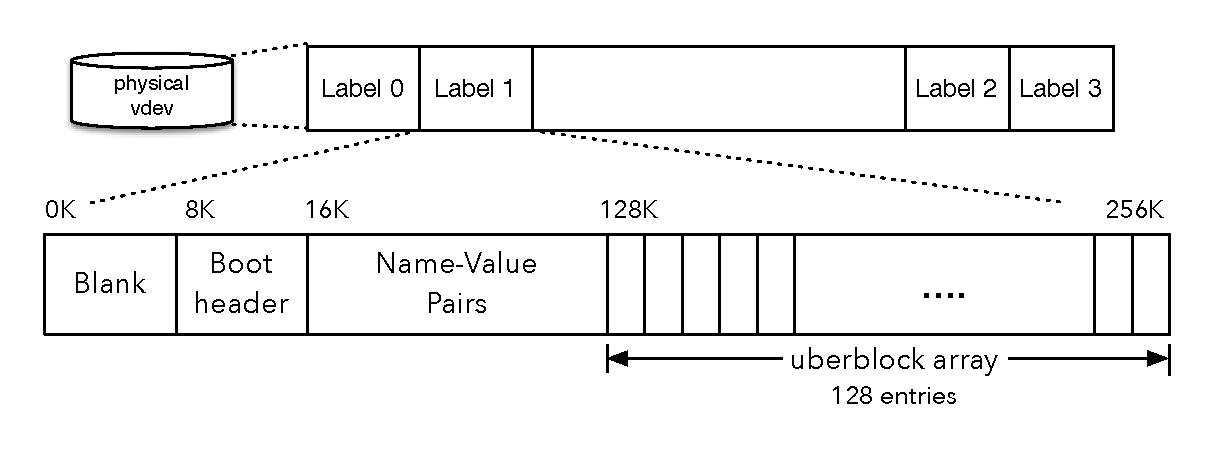
\includegraphics[width=\textwidth]{fig/zfs_vdev_label.pdf}
  \caption{Vdev Label}\label{fig:vlabel}
\end{figure}

\subsubsection{块指针}
除位于固定位置的元数据vdev label外,
所有其它数据位置都是动态分配的,
访问它们都必须通过块指针。
确切地说,
块指针是一个数据块的描述子,
除了记载块在磁盘上的逻辑地址以外,
还有较验和,块类型等域,
块指针结构如\,\ref{fig:blkptr}\,所示。

\begin{figure}[ht]
  \centering
  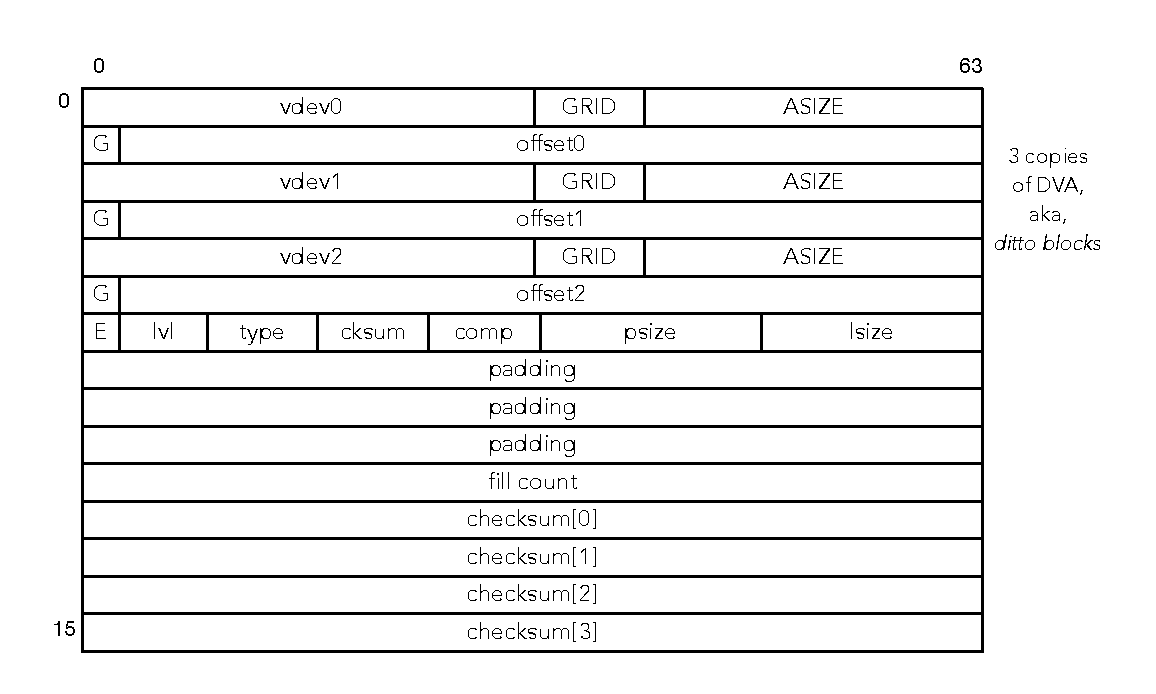
\includegraphics[width=\textwidth]{fig/zfs_blkptr.pdf}
  \caption{Vdev Label}\label{fig:blkptr}
\end{figure}

值得一提的是一个数据块在磁盘上最多可以有三个备份,
ZFS术语称为{\em ditto blocks}。
Uberblock结构有一个\verb|ub_rootbp|域,
游历文件系统数据块就从那里开始。

\subsubsection{对象}
若干数据块以一定方式组织成为对象({\em Object}),
如面向用户的POSIX文件对象(\verb|DMU_OT_PLA-IN_FILE_CONTENTS|)%
和POSIX目录对象(\verb|DMU_OT_DIRECTORY_CONTENTS|),
还有维护ZFS内部逻辑用的\verb|DMU_OT_SPACE_MAP|、
\verb|DMU_OT_DNODE|等对象。

对象的描述子称为{\em dnode},
磁盘上结构为\verb|dnode_phys_t|。
粗略地,
可以把 \verb|dnode_phys_t| 看作 一个模版,
各种类型的对象是这个模版的不同实例,
一个dnode描述相关的数据块如何被组织成该类型的对象。
譬如文件对象描述其所有数据块在磁盘中的分布;
又如目录对象描述如何在该目录下根据文件名检索到对应的文件对象。
dnode类型定义如代码段\,\ref{src:dnode}\,所示。
\inputclisting{zfs_src/dnode.h}
              {ZFS对象}{src:dnode}
一个dnode只包含一个块指针,
ZFS数据块最大尺寸128K,
文件数据超过这一尺寸就需要引入间接块,
ZFS支持最多6级间接寻址,
除第一级间接块尺寸为16K可容纳$2^7$个块指针,
其余均可达到块最大限制128K可容纳$2^{10}$个块指针,
可计算出一个对象的最大尺寸为$2^{7 + 7 + 10 \times 5} = 2^{64}$字节。
图\,\ref{fig:dn_ind}\,演示了一个三级间接寻址。
\begin{figure}[!ht]
  \centering
  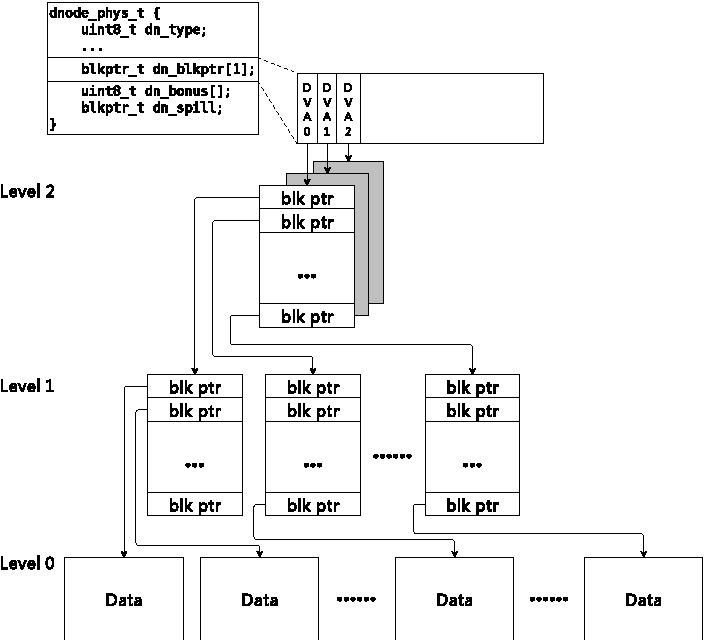
\includegraphics[width=.8\textwidth]{fig/zfs_ind_blkptr.pdf}
  \caption{三级间接寻址}\label{fig:dn_ind}
\end{figure}
              
\subsubsection{对象集}
除了负责将数据块组织成对象,
DMU这一层也管理由多个对象组成的对象集({\em Object Set}。)
换句话说是对象集的数据就是一个个dnode。
对象集有三种,
分别是\verb|DMU_OST_META|、\verb|DMU_OST_ZFS|及\verb|DMU_OST_ZVOL|。
磁盘上描述对象集的数据结构{\em objse\_phys\_t}
定义如代码段\,\ref{src:objset}\,。
\newpage
\inputclisting{zfs_src/objset.h}
              {ZFS对象集}{src:objset}

\begin{figure}[!ht]
  \centering
  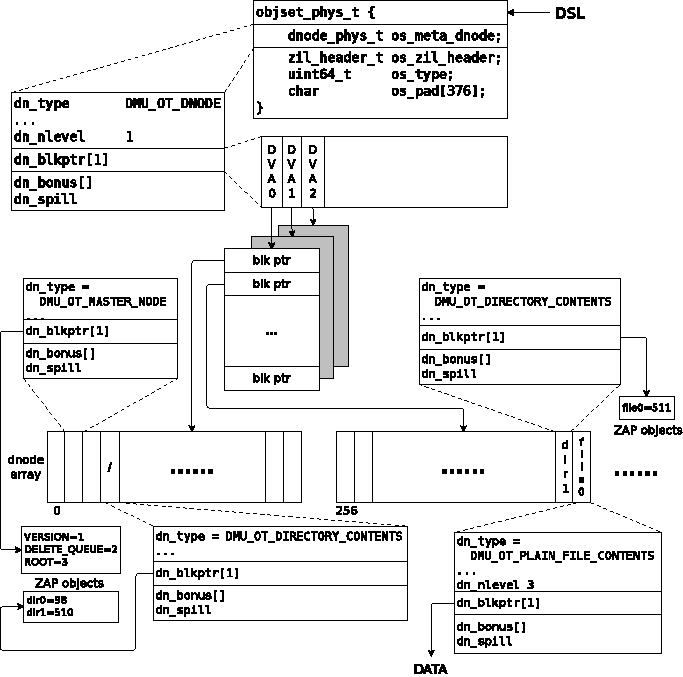
\includegraphics[width=\textwidth]{fig/zfs_objset.pdf}
  \caption{对象集内部组织结构}\label{fig:zfs_objset}
\end{figure}

图\,\ref{fig:zfs_objset}\,示例一个由文件系统对象集定位到指定对象的过程。
从中可以看到,
对象集作为检索对象的起始点,
其结构包含一个dnode类型的域,其类型为\verb|DMU_OT_DNODE|,
换句话说,
该dnode域描述的数据类型为dnode。
另外值得注意的是它的\verb|dn_nlevel|域为1,
说明其描述的dnode寻址树有一级间接寻址。


一个dnode尺寸为512字节,
由上面的计算可知,
一个对象集最多可以容纳$2^{64} / 2^{9} = 2^{55}$个对象。
对象集的数据\,---\,dnode以数组形式存储索引,
每个对象在dnode array中有一个唯一索引号。
索引号为1的dnode有特殊用途,
视对象集的类型而定。
对文件系统类型来说,
该特殊dnode所描述的对象为\verb|DMU_OT_MASTER_NODE|类型,
即一种ZAP对象,
其数据块中存储的信息包括了根目录对象在数组中的索引号,
图中那个``\verb|ROOT=3|''项。
从这里开始就可以遍历访问整个文件系统。
注意到目录类型的对象存储的都是 name-value 对,
value 部分就是对应该名字的dnode在数组中的索引
图中接地的那部分就进入上一节描述的游历一个对象的所有数据块过程。

\subsubsection{DSL}

\begin{figure}[!ht]
  \centering
  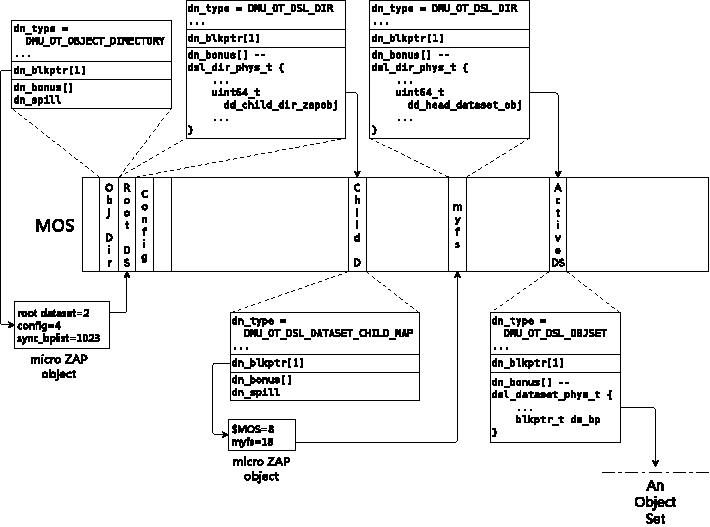
\includegraphics[width=.95\textwidth]{fig/zfs_dsl.pdf}
  \caption{MOS dnode数组结构}\label{fig:mos}
\end{figure}

如何检索到到一个指定的对象集由DSL层负责。
DSL层在磁盘上也呈现为一个对象集,
也就是说它所存储处理的数据也是对象描述子\,--dnode,
这一层对象集的类型为\verb|DMU_OST_META|,
即所谓MOS({\em Meta Object Set}),
MOS也是一个dnode数组。
作为目录项,
MOS中很多项的块指针指向的ZAP对象中存储的是另外某些项在数组中索引的位置,
如图\,\ref{fig:mos}\,中的{\em Object Directory}项描述的数据对象中的%
``root dataset=2'',
又如{\em Child Directory}项数据中的%
``myfs=18''。

在刚引入dnode概念的时候有一个细节没有提及,
就是\verb|dn_bonus|域,
该域有时被用来存储比较小的数据避免分配一个大块。
\footnote{{\tt dmu\_bonus\_hold}函数是个好例子。}
例如图\,\ref{fig:mos}\,中,
文件系统dnode为存储管理活跃的数据集的dnode在MOS的索引没有动用块指针那套机制,
而是在\verb|dn_bonus|中存储\verb|dsl_dir_phys_t|的结构,
这个结构的\verb|dd_head_dataset_obj|域就是当前活跃数据集的dnode在MOS中的索引值;
又如描述活跃对象集的dnode的\verb|dn_bonus|域中存储的是%
\verb|dsl_dataset_phys_t|结构,
通过这个结构的\verb|ds_dp|域指向的数据块即可进入由对象集向对象的检索阶段。
无法将下一层的\verb|objset_phys_t|也嵌入到\verb|dn_bonus|中因为%
\verb|objset_phys_t|本身含有一个dnode结构,
不得已只好开一个块来存储它。

MOS如何寻址得到呢?
答案就是Uberblock。
图\,\ref{fig:uber}\,示意如何完成在磁盘上寻址MOS。
如前所述,
vdev label和uberblock作为整个检索树的根,
必须位于磁盘的固定位置为软件层预先知晓。
\begin{figure}[!hb]
  \centering
  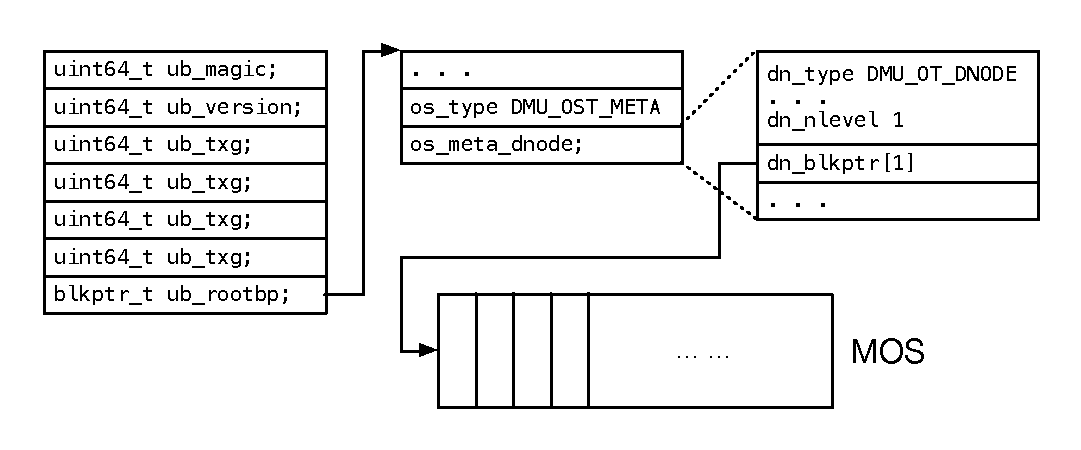
\includegraphics[width=.95\textwidth]{fig/zfs_uber_to_mos.pdf}
  \caption{由Uberblock到MOS}\label{fig:uber}
\end{figure}

\subsection{ZFS块管理---{\em Space Map}}
\subsubsection{位图}
传统的块管理一般使用位图,
思路简单,
一个位表示一个块,
一个字节可以表示8个块,
如果采用4K块大小,
在1T的磁盘上,
需要32M字节的位图,
1PB就需要32G字节,
空间使用和扫描位图的时间开销开始不可接受。
为优化扫描效率,
一个看似可行的方案是将位图分区,
每一个区维护一个整数纪录该区的空闲块数量,
这避免了每一次都扫描整个大位图而只需扫描一个小分区,
譬如1PB的大位图可以分成1M个区。
但这方案仍然有个大问题,
不但分配块需要读写位图,
释放块一样需要。
譬如在1PB的文件系统中删除一个4GB的文件,
需要释放1M个块,
也就是说修改1M个位,
如果运气不好,
上述的1M个位图分区都要被访问到,
这开销太大。
另外当内存容纳不下整个位图,
随机地分配和释放块伴随的位图更新操作将导致大量的磁盘写入。

\subsubsection{B-树}
B-树方案就是在磁盘上存储一棵以{\em extent}%
(即一个起始地址和从那开始的长度)为key的B-树,
这解决一个问题,
就是一次分配或释放一个大连续块组,
只做少数的几个磁盘写入即可更新块管理数据结构,
比位图的一一对应效率高了很多。
大量随机分配释放小块使得在树的各个节点都要更新,
也没有大的extent,
都是描述小extent的节点,
巨额开销仍无法避免。

\subsubsection{延迟释放}
对上述两种数据结构可以做一个优化就是延迟释放,
以期未来某个时候需要分配一个新块的时候直接交付,
直到释放块的数量达到一个阈值对要释放的块地址进行排序,
按顺序更新磁盘上的位图或树,
大大降低了开销。

\subsubsection{Space Map}
ZFS则创新地采用类似log结构的方式存储磁盘块使用信息,
称为{\em Space Map}。Jeff Bonwick在他的博客中提到:

\begin{quotation}
  Recall that log-structured filesystems long  ago posed this question: what if,
  instead of periodically folding a transaction log back into the filesystem, we
  made the transaction log be the filesystem?

  Well, the  same question could  be asked of our  deferred free list:  what if,
  instead of folding it into a bitmap  or B-tree, we made the deferred free list
  be the free space representation?
\end{quotation}

ZFS的确就是这么做的。
ZFS把物理设备划分为一百多个slab,
每个slab有一个块管理数据结构 space map,
当分配或释放某个extent时,
就往space map中追加一条log记录下这一事件,
因为它总是以追加方式记录,
并且由于采用了延迟释放,
随机释放和连续释放效率一样,

另外一个美妙的地方在于当加载一个存储池时,
space map会在内存中表现为一棵按磁盘上地址排序的AVL树,
其节点就是所有空闲块的extent。
这样常常可以将多条log抵消,
或合并为一个节点,
使得树并不很大,
在分配和释放过程中AVL也时不时合并和拆分节点,
再将space map写回磁盘去也不会太大。
极端的例子就是加载一个全满和全空的在内存中AVL树结构一样,
就一个节点。


\subsection{ZFS I/O流水线}
\subsubsection{zfs\_write}
\begin{figure}[!h]
  \centering
  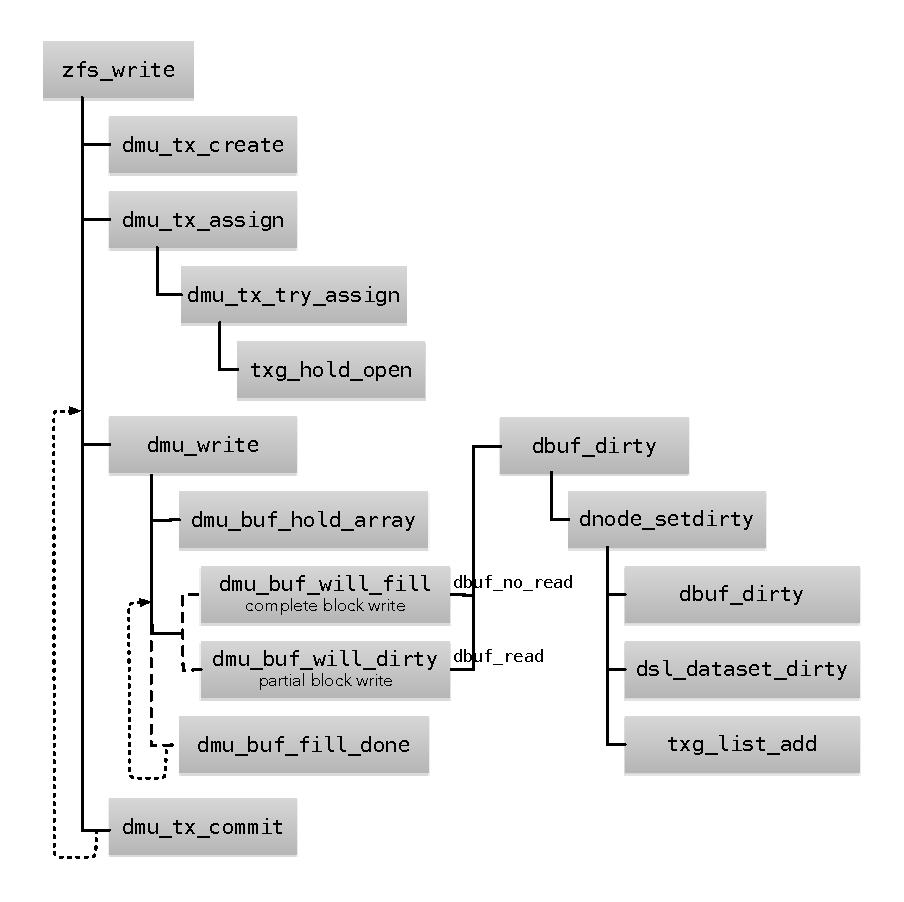
\includegraphics[scale=0.85]{fig/zfs_write.pdf}
  \caption{ZFS 写请求处理流程}\label{fig:zfs_write}
\end{figure}

系统调用和ZFS在写操作方面的交界点在\verb|zfs_write|函数,
此函数从用户空间获取数据并传给DMU层完成写入。
如果用户数据量大就需要将数据分成多个块,
为每一个块开启一个事务,
将事务加入事务组,
写数据块将触发一系列上游节点数据的更新,
将所有的更新都加入同一事务组。
大致调用链如图\,\ref{fig:zfs_write}\,所示。
最后一步提交事务,
负责处理事务组的线程被唤醒,
将事务取下,
完成对物理设备的写入工作。

\subsubsection{事务组}
一个事务组经历三个状态,
\begin{itemize}
  \item open: 新创建事务组即处于open状态,
    对内存中数据结构的更新在这状态中完成
  \item quiescing: 一个缓冲状态,
    这个状态的目的是等待所有组内的事务被提交,
    即过了此阶段,
    不会再有新的事务进入这个事务组,
    一般处于这个状态的事件都很短暂
  \item syncing: 在这个状态,
    将内存中更新写入永久存储介质
\end{itemize}

当创建或加载一个存储池时,
两个事务组线程被创建,
一个负责quiesce,
另一个负责sync。

负责sync的线程被唤醒之后调用\verb|spa_sync|函数,
从这个点到最后触发zio的调用链如图\,\ref{fig:spa_sync}\,所示。
\verb|dsl_pool_sync| 中 \verb|dsl_dataset_sync| 被调用了两次,
每一次都阻塞等带 I/O 返回,
在这一步 I/O 失败被认为是很严重事件,
kernel panic。

\begin{figure}[!ht]
  \centering
  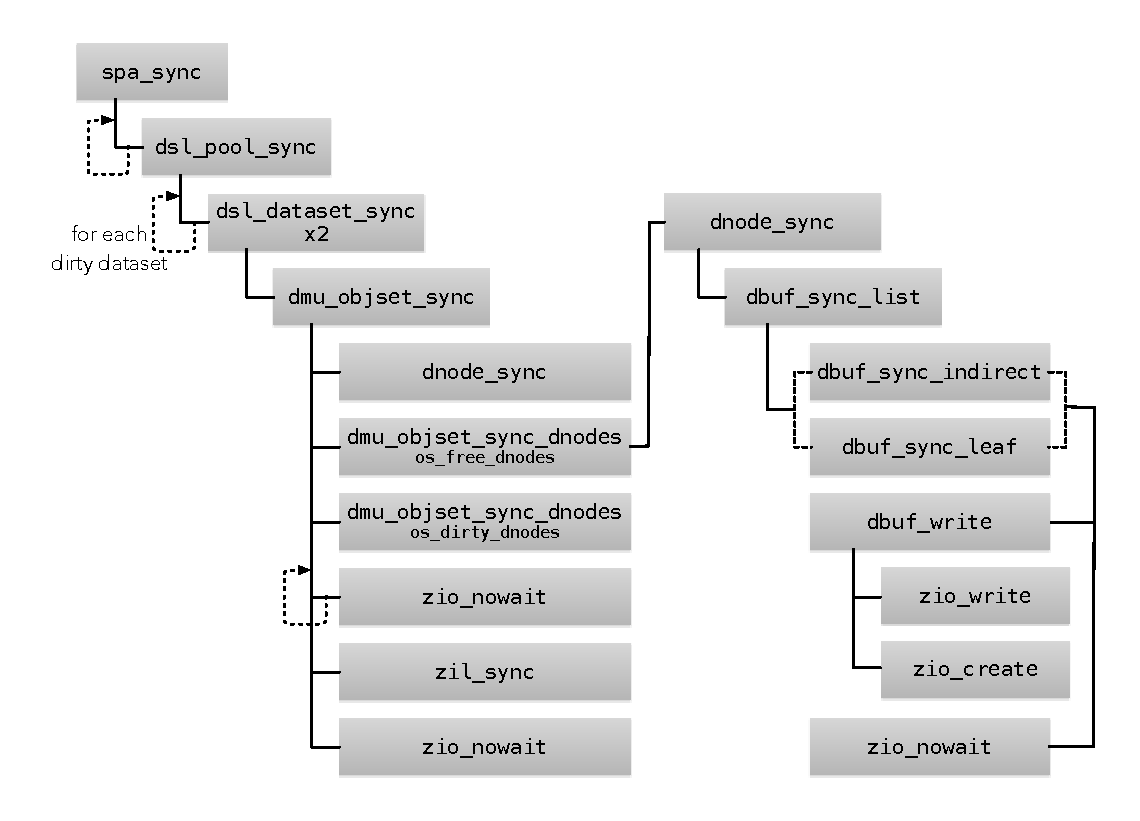
\includegraphics[width=\textwidth]{fig/zfs_spa_sync.pdf}
  \caption{sync到zio的流程}\label{fig:spa_sync}
\end{figure}

\verb|dbuf_sync_leaf|将数据异步地写出。
为了支持 COW,
数据块更新几次,
间接块必须相应更新几次。
\verb|dbuf_sync_indirect|函数对间接块进行读、修改其内容,
创建 ZIO 而后执行写出。

\subsubsection{I/O流水线}
执行 ZIO 的线程不是将整个I/O过程从头至尾执行,
为了提高吞吐率,
充分利用多核特性,
I/O被分为多道工序,
以优化方式分配给流水线上的工作线程。

I/O操作分为五类,
\begin{enumerate*}[label=\itshape\arabic*\upshape)]
  \item Read
  \item Write
  \item Free
  \item Claim
  \item Ioctl
\end{enumerate*}
这五类操作由不同的工序按指定顺序组合而成。

ZIO流水线的核心函数是\verb|zio_execute|。
和工厂流水线上工人一人只负责某几道确定工序不同,
ZIO 的线程可以负责任意工序,
一个线程完成某道工序之后有两种可能,
如果工序例程调用\verb|zio_taskq_dispatch|将
将半成品挂到某个队列上返回\verb|ZIO_PIPELINE_STOP|,
\verb|zio_execute|停止执行,返回,
之后工序交给谁处理由上一层逻辑按优化方式决定(当然可能还是同一个线程);%
\footnote{这里可能有优化余地,
  即让线程自己根据优化逻辑决定是挂出半成品还是自己继续处理}
否则例程会返回\verb|ZIO_PIPELINE_CONTINUE|,
当前线程在\verb|zio_execute|中继续调用下一道工序例程。

Write:
举例来说,
写操作的流水线定义如下:

\begin{lstlisting}{lanuage=C}
#define ZIO_WRITE_COMMON_STAGES		\
        (ZIO_INTERLOCK_STAGES	|	\
         ZIO_VDEV_IO_STAGES	|	\
         ZIO_STAGE_ISSUE_ASYNC	|	\
         ZIO_STAGE_CHECKSUM_GENERATE)
\end{lstlisting}

根据定义:

\begin{lstlisting}{lanuage=C}
 ZIO_STAGE_READY		= 1 << 16,	/* RWFCI */
 ZIO_STAGE_DONE			= 1 << 21,	/* RWFCI */
 ZIO_STAGE_VDEV_IO_START	= 1 << 17,	/* RWF-I */
 ZIO_STAGE_VDEV_IO_DONE		= 1 << 18,	/* RWF-- */
 ZIO_STAGE_VDEV_IO_ASSESS	= 1 << 19,	/* RWF-I */
 ZIO_STAGE_ISSUE_ASYNC		= 1 << 3,	/* RWF-- */
 ZIO_STAGE_CHECKSUM_GENERATE	= 1 << 5,	/* -W--- */
\end{lstlisting}

各道工序的例程在\verb|zio_pipeline|中定义:
\begin{lstlisting}{language=C}
static zio_pipe_stage_t *zio_pipeline[] = {
	NULL,
	zio_read_bp_init,
	zio_free_bp_init,
	zio_issue_async,
	zio_write_bp_init,
	zio_checksum_generate,
	zio_nop_write,
	zio_ddt_read_start,
	zio_ddt_read_done,
	zio_ddt_write,
	zio_ddt_free,
	zio_gang_assemble,
	zio_gang_issue,
	zio_dva_allocate,
	zio_dva_free,
	zio_dva_claim,
	zio_ready,
	zio_vdev_io_start,
	zio_vdev_io_done,
	zio_vdev_io_assess,
	zio_checksum_verify,
	zio_done
};
\end{lstlisting}

也就是说要完成\verb|zio_write|,
以下流水线上函数将被依次调用:
\begin{lstlisting}{lanuage=C}
 zio_issue_async,
 zio_checksum_generate,
 zio_ready,
 zio_vdev_io_start,
 zio_vdev_io_done,
 zio_vdev_io_assess,
 zio_done
\end{lstlisting}

\verb|zio_issue_async|函数将zio挂如一个taskq线程的队列,
告知\verb|zio_execute|立即返回,
taskq线程完成余下工作。

\verb|zio_checksum_generate|函数生成较验和之后返回
\verb|ZIO_PIPELINE_CONTINUE|,
于是该taskq线程继续下一道工序,即\verb|zio_ready|。

\verb|zio_ready|一开始调用\verb|zio_wait_for_children|,
如果zio有gang或者ddt类型的子zio,
\verb|zio_wait_for_children|将工序移至下一道,
但状态设为{\em stall}并返回stop,
使得\verb|zio_execute|直接返回,
zio的工序暂停,
直至所有子zio都到达\verb|READY|阶段以后才能继续执行。
\verb|zio_ready|将调用\verb|zio_notify_parent|,
\verb|zio_notify_parent|又调用\verb|zio_execute|%
继续父zio刚才暂停的工序,
当然并非一定是该线程完成,
依然可能是将zio挂到某个taskq的队列中就返回。

下一道工序是\verb|zio_vdev_io_start|,
它负责为物理I/O做准备。
如果该zio的vdev是物理设备,
调用\verb|vdev_queue_io|将zio挂入vdev的队列,
返回\verb|STOP|;
否则直接调用该设备的\verb|vdev_op_io_start|%
(可能是mirro,或者Raid等等)
方法将zio逐层下传至物理设备。
这一道工序总是返回\verb|STOP|。

\verb|zio_vdev_op_io_done|主要就是错误处理,
之后就是收尾的两道工序。

\subsubsection{ARC及L2ARC}
LRU:
考虑如下场景,
当程序一次性地读入大量数据(常见的例如:\verb|grep -nr|),
那些数据块轻易填满cache,
挤出大量的页,
但它们仅仅被使用一次,
滞留在cache中毫无益处。
那些被频繁使用的页却被无谓地换出。
另外一方面,
单单考虑页面访问频度的策略也有其缺陷,
ARC的思路是同时采纳两种策略,
并且自适应地在二者间做权衡。

ARC:
ARC维护两个先进先出的页面队列,
分别存放按MRU和MFU策略处理的页描述子。
MRU和MFU还各自有一个ghost队列。
页面第一次被读入并缓存时,
插入MRU队列头部,
当它第二次被访问就移入MFU队列,
在MFU队列中再次被访问则会移到队列头。
当cache够用时,
两个ghost队列都为空,
MFU和MRU各自扩张到最大限度。
如图\,\ref{fig:zfs_arc0}\,所示。

\begin{figure}[!h]
  \centering
  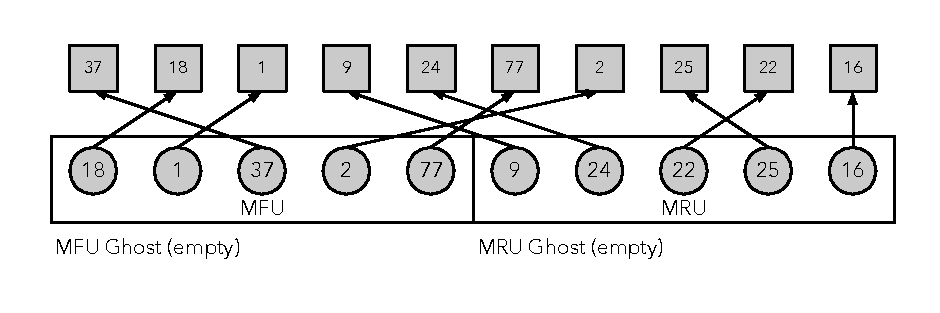
\includegraphics[width=\textwidth]{fig/zfs_arc0.pdf}
  \caption{MSU和MRU}\label{fig:zfs_arc0}
\end{figure}

\begin{figure}[!ht]
  \centering
  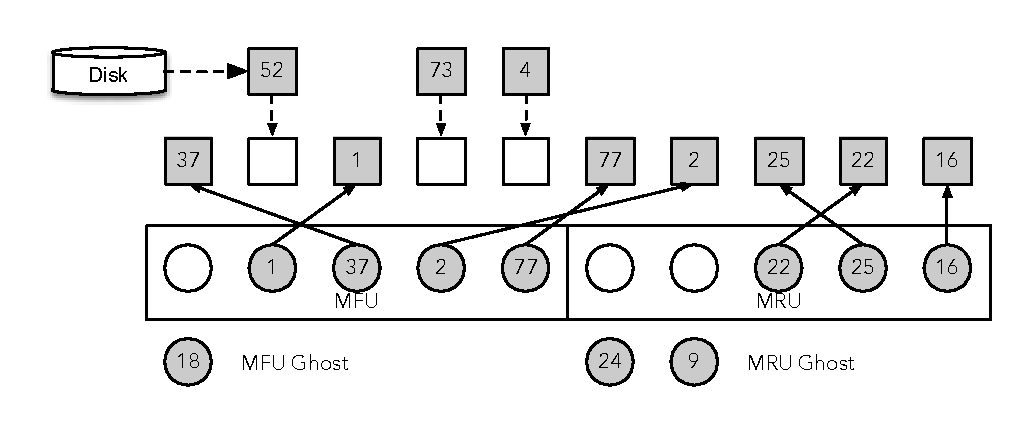
\includegraphics[width=\textwidth]{fig/zfs_arc1.pdf}
  \caption{Evicted to Ghost Lists}\label{fig:zfs_arc1}
\end{figure}

内存紧张以后,
再从磁盘读入新页将触发cache中某些页面被清除({\em evict}),
这时将该页面的描述子插入其所属页缓存类的ghost队列头,
即虽然磁盘数据块已经不在内存中,
其引用依然保留。
当然ghost队列越来越长到达最大限度以后,
页面的描述子将被依次序删除,
对应磁盘数据块的引用彻底消失。
图\,\ref{fig:zfs_arc1}\,演示了页面被evict的场景。

当已换出数据块再次被从磁盘读取,
如果发现其引用仍位于某个的ghost队列中,
这透露的一个信息是该类页缓存的miss率较高,
需要增加该类页缓存的额度,
当然同时减少另外一方的额度,
图\,\ref{fig:zfs_arc2}\,演示了这一过程。

\begin{figure}[!ht]
  \centering
  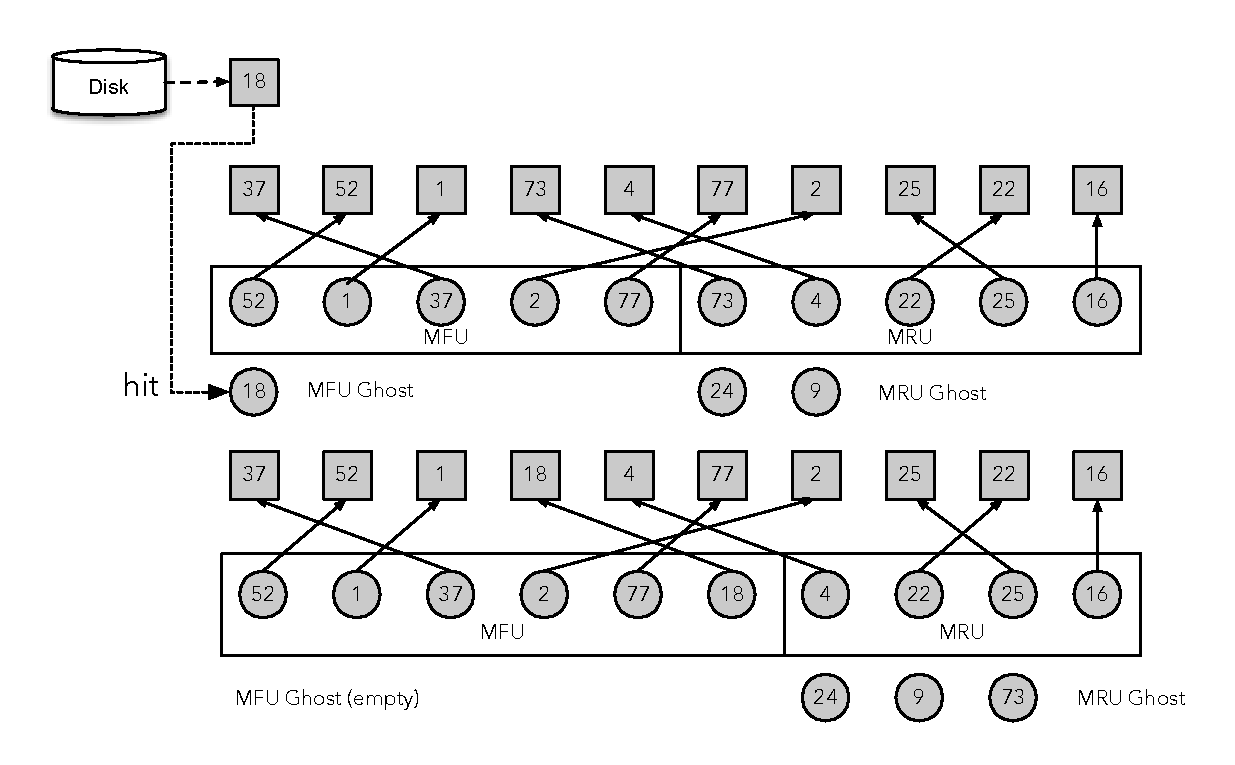
\includegraphics[width=\textwidth]{fig/zfs_arc2.pdf}
  \caption{Expand MFU and Shrink MRU}\label{fig:zfs_arc2}
\end{figure} 

两类页缓存策略采用相同的逻辑,
两种策略自适应地趋向符合work load的页使用需求。
仍然考虑之前的场景,
一次性读入大量数据导致MRU的ghost队列很长,
但它们再没有被命中过,
如果有其它的应用%
\footnote{譬如数据库在某些时候会反复执行相同的查询}%
使得MFU的ghost队列总是命中,
于是MFU的页缓存队列越来越长而MRU的页缓存队列越来越短,
逐渐达到平衡,
页面的换出策略得到优化。

ZFS对ARC的实现与源算法有些小区别。
\begin{itemize}
  \item ZFS 的缓存容量根据当前可用内存动态可变;
  \item ZFS 支持多种不同块尺寸;
  \item ZFS 支持把一个页锁在内存中,
    在清除页时需要扫一下队列找最老的可清除的页。
\end{itemize}

L2ARC:
可以让ZFS使用SSD作为二级页缓存设备,
即所谓{\em L2ARC},
它使用了一个\verb|l2arc_only|队列维护只在SSD上的页缓存。
其主要算法和ARC完全一致。
一个自然的想法使当ARC需要清除页面时,
自动地清到SSD上。
但这样将导致一些严重问题,
其一是当有一个大数据读将一次刷出大量页面到SSD上,
其二是当应用程序开辟大量内存是,
ARC需要被缩减,这时又可能导致一次性大量页面刷出。
ZFS解决方法是用一个线程\verb|l2arc_feed_thread|扫描两个缓存队列,
将最近可能要清除出去的页组到一个8M的缓冲区,
之后由另一个\verb|write_hand|线程一次性写出,
这适当降低了突发大量写的危害。


\subsubsection{Solaris fd space}
随着进程打开关闭文件,
内核时不时分配释放fd,
fd空间就会出现很多空洞。
由于历史原因,
打开文件分配fd时总是从当前可用的fd中找最小的那一个,
要快速地从中找出第一个可用的fd是一个挑战。
显然进程的fd空间[0\dots {\sc max\_fd}]可看作一棵完全二叉检索树的中序遍历,
找最小fd的过程可看作遍历二叉树在其中找一个最小的空闲节点。
方法是每个节点维护以该节点包括它子集的右子树中已分配的fd数,
通过判断当前树是否完全和右子树已分配节点数可以决定搜寻方向。
巧妙地利用二进制数的性质可以快速计算父子以及当树完全时某子树的节点数。
这样由[0\dots {\sc max\_fd}]数组表示完全二叉检索树有以下一系列属性:

\begin{enumerate}
\item 树中节点的最低被置位的位置指示该节点位于树中的第几层,
  譬如x1位于最底层 ,
  x10节点位于树的第一层,
  并且同一层的节点值从左向右递增;
  
\item 节点的右子树的节点包括它本身的个数($csize$)
  等于将该节点值仅保留最低被置位所得的值,
  譬如x10右子树的所有节点数$csize(\text{x10})$为2;
  
\item 节点$n$的最近左祖先(即$n$位于它的右子树中)
  $lparent$等于清除该节点的最低被置位,
  因为$lparent(n)$是清除最低被置位,
  而$csize(n)$是清除除最低被置位外的所有位,
  所以$lparent(n) = n - csize(n)$;
  
\item 最近的右祖先$rparent(n) = n + csize(n)$

\item 任意内部节点,
  子和父值之差为$csize(parent) / 2$。
\end{enumerate}

根据:
\begin{eqnarray}
  n &=& \textit{xxxx10}\dots{\it 0}\\
  n - 1 &=& \textit{xxxx01}\dots{\it 1}\\
  n \;\&\; (n - 1) &=& \textit{xxxx00}\dots{\it 0}\\
  n \,\mid\, (n - 1) &=& \textit{xxxx11}\dots{\it 1}\\
  n \,\XOR\, (n - 1) &=& \textit{000011}\dots{\it 1}
\end{eqnarray}

可以快速地计算出:
\begin{eqnarray}
  csize(n) &=& (n - 1) \,\XOR\, (n \,\mid\, (n - 1))\\
  lparent(n) &=& n \;\&\; (n - 1)\\
  rparent(n) &=& (n \,\mid\, (n − 1)) + 1
\end{eqnarray}

考虑到fd从0开始,
公式中变量值由$n$变为$n' = n - 1$,
并且计算出的fd值要减去1,
于是真正实现中使用的公式为:

\begin{eqnarray}
  csize(n) &=& n \,\XOR\, (n \,\mid\, (n + 1))\\
  lparent(n) &=& n \;\&\; (n + 1) - 1\\
  rparent(n) &=& (n \,\mid\, (n + 1))
\end{eqnarray}

具体到代码实现,
\struct{proc\_t.p\_user.u\_finfo.fi\_list}就是进程的fd空间数组,
数组元素类型为\struct{uf\_entry},
数组元素逻辑上看作二叉树中的一个节点,
数组索引$n$就是节点值,
域\struct{uf\_alloc}被用于存储节点$n$当前右子树(包括它自己)的总节点数,
如果\struct{uf\_alloc}不等于$csize(n)$,
说明在它的右子树里至少有一个fd可用。

函数\func{fd\_find}接受一个minfd参数,
完成搜寻$\ge\,$minfd的fd中最小的那一个。
打开文件时通常传入0作为minfd参数。
搜寻的过程如下:
\begin{enumerate}
\item 从以minfd为根的树找起,
  计算$csize(minfd)$,
  和\struct{fi\_list[minfd].uf\_alloc}比较,
  如果不等,
  说明在minfd的右子树下可以找到一个空闲的fd,这一步结束;
  否则上溯到minfd的右祖先,
  继续这一步直至找到某个节点fd满足$csize(fd)$不等于
  \struct{fi\_list[fd].uf\_alloc};
\item 从上一步得到的节点为根,
  开始搜寻树中最小的空闲fd,
  查左子树而后右子树。
\end{enumerate}

\inputclisting{snippet/fio.c}
              {fd space management}{fdspace}

\func{fd\_find}只负责找到一个可用fd值,
\func{fd\_reserve}真正进行fd的分配或释放工作,
完成之后函数要从节点一直上溯到最左祖先,
更新它们的右子树已分配节点数。
